\documentclass[12pt,a4paper]{report}

% Encodage et langue
\usepackage[utf8]{inputenc}
\usepackage[T1]{fontenc}
\usepackage[french]{babel}

% Mise en page
\usepackage[margin=2.5cm]{geometry}
\usepackage{setspace}
\onehalfspacing

% Graphiques et images
\usepackage{graphicx}
\graphicspath{{images/}}
\usepackage{float}

% Code source
\usepackage{listings}
\usepackage{xcolor}

\definecolor{codegreen}{rgb}{0,0.6,0}
\definecolor{codegray}{rgb}{0.5,0.5,0.5}
\definecolor{codepurple}{rgb}{0.58,0,0.82}
\definecolor{backcolour}{rgb}{0.95,0.95,0.95}

\lstdefinestyle{mystyle}{
    backgroundcolor=\color{backcolour},
    commentstyle=\color{codegreen},
    keywordstyle=\color{codepurple},
    numberstyle=\tiny\color{codegray},
    stringstyle=\color{codegreen},
    basicstyle=\ttfamily\footnotesize,
    breakatwhitespace=false,
    breaklines=true,
    captionpos=b,
    keepspaces=true,
    numbers=left,
    numbersep=5pt,
    showspaces=false,
    showstringspaces=false,
    showtabs=false,
    tabsize=2,
    frame=single
}
\lstset{style=mystyle}

% Liens
\usepackage{hyperref}
\hypersetup{
    colorlinks=true,
    linkcolor=blue,
    filecolor=magenta,
    urlcolor=cyan,
    citecolor=blue
}

% Tableaux
\usepackage{booktabs}
\usepackage{tabularx}
\usepackage{longtable}

% Divers
\usepackage{enumitem}
\usepackage{fancyhdr}
\usepackage{titlesec}

% En-tete et pied de page
\pagestyle{fancy}
\fancyhf{}
\rhead{DEUS Dashboard}
\lhead{EPITA --- Projet DevOps}
\rfoot{Page \thepage}

% Bibliographie
\usepackage[backend=biber,style=numeric]{biblatex}
\addbibresource{bibliography.bib}

% ============================
\begin{document}

% Page de titre
\begin{titlepage}
    \centering
    \vspace*{2cm}

    {\Huge\bfseries DEUS Dashboard\par}
    \vspace{0.5cm}
    {\Large Deploiement DevOps sur AWS\par}
    \vspace{2cm}

    {\large\itshape Michael Rousseau\par}
    \vspace{1cm}

    {\large EPITA --- Cycle Ingenieur 2\textsuperscript{e} annee\par}
    \vspace{0.5cm}
    {\large Module DEUS\par}
    \vspace{2cm}

    {\large \today\par}
    \vspace{2cm}

    \begin{abstract}
        Ce rapport presente la mise en place d'une infrastructure DevOps complete
        pour le deploiement d'une application web Angular sur Amazon Web Services.
        Le projet couvre l'ensemble de la chaine DevOps~: conteneurisation avec Docker,
        infrastructure as code avec Terraform, gestion de configuration avec Ansible,
        integration et deploiement continus avec GitHub Actions, monitoring avec CloudWatch,
        et gestion des secrets avec SSM Parameter Store.
    \end{abstract}
\end{titlepage}

\tableofcontents
\newpage

\chapter{Introduction}

\section{Contexte du projet}

Le projet DEUS Dashboard est une application web permettant de visualiser des donnees
astronomiques fournies par les APIs de la NASA. L'application affiche l'image astronomique
du jour (APOD), les evenements naturels terrestres (EONET), ainsi qu'une carte interactive
de la Lune.

L'objectif de ce projet est de mettre en \oe{}uvre une methodologie DevOps complete
pour deployer cette application sur Amazon Web Services (AWS), en demontrant la maitrise
des outils et pratiques essentiels du domaine.

\section{Objectifs}

\begin{itemize}
    \item Conteneuriser l'application avec Docker
    \item Provisionner l'infrastructure AWS avec Terraform (Infrastructure as Code)
    \item Configurer les serveurs avec Ansible (Configuration Management)
    \item Automatiser les deploiements avec GitHub Actions (CI/CD)
    \item Mettre en place un monitoring avec CloudWatch
    \item Securiser l'infrastructure (IAM, VPC, SSM Parameter Store)
\end{itemize}

\section{Technologies utilisees}

\begin{table}[H]
    \centering
    \begin{tabularx}{\textwidth}{lX}
        \toprule
        \textbf{Categorie} & \textbf{Technologies} \\
        \midrule
        Frontend & Angular 20, TypeScript, Leaflet \\
        Backend & Node.js, Express 5, TypeScript \\
        Base de donnees & PostgreSQL 16 (RDS), DynamoDB \\
        Conteneurisation & Docker, Docker Compose \\
        Infrastructure & Terraform, AWS (VPC, ECS, ALB, S3, CloudFront) \\
        Configuration & Ansible \\
        CI/CD & GitHub Actions \\
        Monitoring & CloudWatch (Logs, Metriques, Alarmes, Dashboard) \\
        Securite & IAM, Security Groups, SSM Parameter Store \\
        \bottomrule
    \end{tabularx}
    \caption{Stack technologique du projet}
\end{table}

\chapter{Architecture}

\section{Vue d'ensemble}

L'architecture suit un modele cloud-native avec separation entre le frontend statique
et le backend API.

% TODO: Remplacer par une capture d'ecran du diagramme d'architecture
% \begin{figure}[H]
%     \centering
%     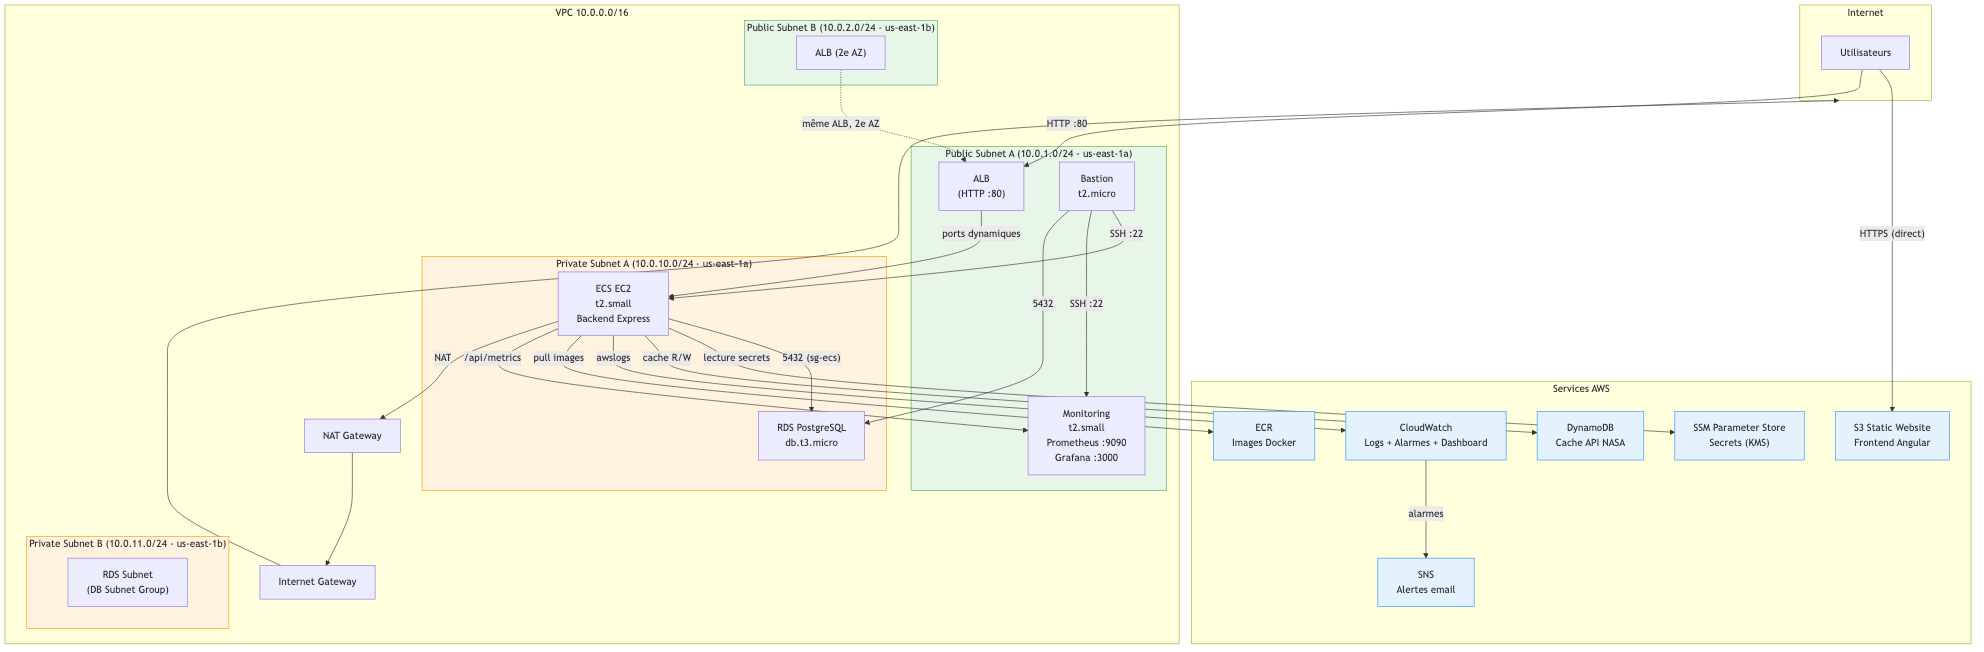
\includegraphics[width=\textwidth]{architecture-diagram.png}
%     \caption{Diagramme d'architecture globale}
% \end{figure}

\begin{lstlisting}[language={},caption={Architecture simplifiee}]
   Utilisateurs --> CloudFront --> S3 (Angular)
   Utilisateurs --> ALB --> ECS (EC2) --> Express Backend
                                |              |
                           RDS PostgreSQL   DynamoDB (cache)

   SSM Parameter Store <-- secrets
   CloudWatch <-- logs, metriques, alarmes
\end{lstlisting}

\section{Composants}

\subsection{Frontend --- S3 + CloudFront}

L'application Angular est compilee en fichiers statiques et deployee sur un bucket S3.
CloudFront sert de CDN avec~:
\begin{itemize}
    \item Origin Access Control (OAC) pour securiser l'acces au bucket
    \item Redirection HTTPS automatique
    \item Gestion du routage SPA (erreurs 403/404 redirigees vers \texttt{index.html})
\end{itemize}

\subsection{Backend --- ECS (EC2 Launch Type)}

Le backend Express est conteneurise et deploye sur ECS avec le type de lancement EC2.
Ce choix, plutot que Fargate, permet de~:
\begin{itemize}
    \item Configurer les instances EC2 avec Ansible
    \item Demontrer la gestion de l'Auto Scaling Group
    \item Installer des agents de monitoring personnalises
\end{itemize}

Un Application Load Balancer (ALB) distribue le trafic vers les conteneurs
via le port mapping dynamique.

\subsection{Bases de donnees}

\begin{description}
    \item[RDS PostgreSQL] Base relationnelle pour les favoris utilisateur et l'historique
        de recherche. Instance \texttt{db.t3.micro} en single-AZ.
    \item[DynamoDB] Cache des reponses API NASA avec TTL automatique.
        Mode de facturation PAY\_PER\_REQUEST.
\end{description}

\section{Choix d'architecture}

\begin{table}[H]
    \centering
    \begin{tabularx}{\textwidth}{lXl}
        \toprule
        \textbf{Decision} & \textbf{Justification} & \textbf{Alternative} \\
        \midrule
        ECS EC2 vs Fargate & Permet Ansible, plus pedagogique & Fargate \\
        Bridge networking & Standard EC2, port mapping dynamique & awsvpc \\
        Single NAT Gateway & Economie (\~{}32\$/mois) & HA NAT \\
        PriceClass\_100 & Regions US/EU suffisantes & PriceClass\_All \\
        Single-AZ RDS & Projet scolaire, economie & Multi-AZ \\
        \bottomrule
    \end{tabularx}
    \caption{Decisions d'architecture et justifications}
\end{table}

\section{Reseau --- VPC}

\begin{table}[H]
    \centering
    \begin{tabular}{llll}
        \toprule
        \textbf{Sous-reseau} & \textbf{CIDR} & \textbf{AZ} & \textbf{Usage} \\
        \midrule
        public\_a & 10.0.1.0/24 & us-east-1a & ALB, Bastion \\
        public\_b & 10.0.2.0/24 & us-east-1b & ALB (2\textsuperscript{e} AZ) \\
        private\_a & 10.0.10.0/24 & us-east-1a & ECS, RDS \\
        private\_b & 10.0.11.0/24 & us-east-1b & Groupe RDS \\
        \bottomrule
    \end{tabular}
    \caption{Allocation des sous-reseaux}
\end{table}

\chapter{Backend API}

\section{Presentation}

Le backend est une API REST construite avec Express 5 et TypeScript. Son role principal
est de servir de proxy securise vers les APIs NASA, en cachant la cle API cote serveur.

\section{Structure du projet}

\begin{lstlisting}[language={},caption={Arborescence du backend}]
backend/
  src/
    index.ts           # Point d'entree
    app.ts             # Configuration Express
    config/
      index.ts         # Variables d'environnement
      database.ts      # Pool PostgreSQL
      dynamodb.ts      # Client DynamoDB
    routes/
      health.ts        # GET /api/health
      apod.ts          # GET /api/apod, /range, /random
      events.ts        # GET /api/events
      favorites.ts     # CRUD /api/favorites
    services/
      nasaApi.service.ts  # Appels HTTP vers NASA
      cache.service.ts    # Cache DynamoDB
    middleware/
      errorHandler.ts
\end{lstlisting}

\section{Routes API}

\begin{table}[H]
    \centering
    \begin{tabularx}{\textwidth}{llXl}
        \toprule
        \textbf{Methode} & \textbf{Route} & \textbf{Description} & \textbf{Cache} \\
        \midrule
        GET & /api/health & Verification de sante & Non \\
        GET & /api/apod & Image du jour & DynamoDB \\
        GET & /api/apod/range & Images par plage de dates & DynamoDB \\
        GET & /api/apod/random & Images aleatoires & Non \\
        GET & /api/events & Evenements naturels & DynamoDB \\
        GET & /api/favorites & Liste des favoris & Non \\
        POST & /api/favorites & Ajouter un favori & Non \\
        DELETE & /api/favorites/:date & Supprimer un favori & Non \\
        \bottomrule
    \end{tabularx}
    \caption{Endpoints de l'API}
\end{table}

\section{Dockerfile}

Le Dockerfile utilise un build multi-stage pour minimiser la taille de l'image~:

\begin{lstlisting}[language=bash,caption={Dockerfile multi-stage}]
FROM node:20-alpine AS builder
WORKDIR /app
COPY package*.json ./
RUN npm ci
COPY tsconfig.json ./
COPY src/ ./src/
RUN npm run build

FROM node:20-alpine
WORKDIR /app
RUN addgroup -g 1001 appgroup && \
    adduser -u 1001 -G appgroup -s /bin/sh -D appuser
COPY --from=builder /app/dist ./dist
COPY --from=builder /app/package*.json ./
RUN npm ci --omit=dev
USER appuser
EXPOSE 3000
CMD ["node", "dist/index.js"]
\end{lstlisting}

Points cles~:
\begin{itemize}
    \item Utilisateur non-root (\texttt{appuser}) pour la securite
    \item \texttt{npm ci --omit=dev} en production pour reduire la taille
    \item Base \texttt{node:20-alpine} pour une image legere (\~{}180 Mo)
\end{itemize}

\section{Docker Compose --- Developpement local}

\begin{lstlisting}[language=bash,caption={Services docker-compose}]
services:
  backend:     # Express API (port 3000)
  postgres:    # PostgreSQL 16 (port 5432)
  dynamodb-local:  # DynamoDB Local (port 8000)
\end{lstlisting}

Le fichier \texttt{docker-compose.yml} a la racine du projet permet de lancer
l'ensemble de la stack localement avec \texttt{docker compose up}.

\chapter{Terraform --- Infrastructure as Code}

\section{Presentation}

Terraform est utilise pour provisionner l'ensemble de l'infrastructure AWS de maniere
declarative et reproductible. La configuration est organisee en modules reutilisables.

\section{Gestion de l'etat}

L'etat Terraform est stocke dans un bucket S3 avec verrouillage DynamoDB~:

\begin{lstlisting}[language=bash,caption={Configuration du backend S3}]
terraform {
  backend "s3" {
    bucket         = "deus-dashboard-tfstate"
    key            = "dev/terraform.tfstate"
    region         = "us-east-1"
    dynamodb_table = "deus-dashboard-tf-locks"
    encrypt        = true
  }
}
\end{lstlisting}

Ce mecanisme garantit~:
\begin{itemize}
    \item Le versionnement de l'etat (historique des changements)
    \item Le verrouillage concurrent (un seul \texttt{apply} a la fois)
    \item Le chiffrement au repos
\end{itemize}

\section{Organisation en modules}

\begin{table}[H]
    \centering
    \begin{tabularx}{\textwidth}{lX}
        \toprule
        \textbf{Module} & \textbf{Ressources} \\
        \midrule
        vpc & VPC, sous-reseaux, IGW, NAT Gateway, tables de routage \\
        s3-cloudfront & Bucket S3, distribution CloudFront, OAC \\
        ecr & Repository ECR, politique de cycle de vie \\
        ecs & Cluster ECS, Launch Template, ASG, ALB, Task Definition, Service \\
        rds & Instance PostgreSQL, sous-groupe DB, Security Group \\
        dynamodb & Table de cache avec TTL \\
        bastion & Instance EC2 t2.micro, Security Group SSH \\
        iam & Roles ECS (execution, task, instance), Instance Profile \\
        ssm & Parametres SecureString (cle NASA, credentials DB) \\
        monitoring & Log Groups, Alarmes CloudWatch, SNS, Dashboard \\
        \bottomrule
    \end{tabularx}
    \caption{Modules Terraform et leurs ressources}
\end{table}

\section{Graphe de dependances}

Les modules sont lies par leurs outputs/inputs~:

\begin{lstlisting}[language={},caption={Ordre de deploiement}]
VPC (base)
  |-- Bastion, ECR, S3/CloudFront, DynamoDB (parallele)
  |-- IAM (apres ECR, DynamoDB)
  |-- RDS (apres VPC, Bastion)
  |-- SSM (apres RDS, DynamoDB)
  |-- ECS (apres tout)
  |-- Monitoring (apres ECS, RDS)
\end{lstlisting}

\section{Variables et secrets}

Les valeurs sensibles sont passees via \texttt{TF\_VAR\_*} en CI
et ne sont jamais commitees dans le code~:

\begin{table}[H]
    \centering
    \begin{tabular}{lll}
        \toprule
        \textbf{Variable} & \textbf{Type} & \textbf{Source} \\
        \midrule
        db\_password & sensitive & GitHub Secret \\
        nasa\_api\_key & sensitive & GitHub Secret \\
        ssh\_key\_name & string & GitHub Variable \\
        \bottomrule
    \end{tabular}
    \caption{Variables sensibles Terraform}
\end{table}

% TODO: Ajouter capture d'ecran terraform plan
% \begin{figure}[H]
%     \centering
%     \includegraphics[width=\textwidth]{terraform-plan.png}
%     \caption{Sortie de terraform plan}
% \end{figure}

\chapter{Ansible --- Configuration Management}

\section{Presentation}

Ansible est utilise pour configurer les instances EC2 qui hebergent les conteneurs ECS.
Il intervient apres le provisionnement Terraform pour installer et configurer~:
\begin{itemize}
    \item Docker et le daemon ECS
    \item L'agent CloudWatch pour les metriques systeme
    \item Le durcissement de securite des instances
\end{itemize}

\section{Inventaire}

L'inventaire est statique (\texttt{inventory/hosts.ini}) et regroupe les
hotes en trois groupes~: \texttt{bastion}, \texttt{ecs\_instances} et
\texttt{monitoring}. Les adresses IP changent a chaque session Learner Lab
(les instances sont recreees ou redemarrees)~; l'inventaire est donc mis a
jour a partir des outputs Terraform (\texttt{bastion\_public\_ip},
IP privees des instances ECS et monitoring).

Les variables communes aux instances ECS (nom du cluster, region, log group)
sont centralisees dans \texttt{inventory/group\_vars/ecs\_instances.yml}
et doivent rester coherentes avec les outputs Terraform.

\section{Roles}

\subsection{Role \texttt{security}}

Durcissement des instances~:
\begin{itemize}
    \item Desactivation du login SSH root
    \item Desactivation de l'authentification par mot de passe
    \item Installation des mises a jour de securite automatiques
    \item Restriction des permissions cron
\end{itemize}

\subsection{Role \texttt{docker}}

Installation et activation de Docker CE sur les instances Amazon Linux 2023.

\subsection{Role \texttt{ecs-agent}}

Configuration de l'agent ECS via le template \texttt{/etc/ecs/ecs.config}
qui specifie le cluster cible et active les metadonnees de conteneur.

\subsection{Role \texttt{cloudwatch-agent}}

Installation de l'agent CloudWatch unifie avec collecte~:
\begin{itemize}
    \item Metriques CPU, memoire, disque
    \item Logs de l'agent ECS (\texttt{/var/log/ecs/ecs-agent.log})
\end{itemize}

\section{Playbook monitoring}

Un second playbook (\texttt{playbooks/monitoring.yml}) configure l'instance
dediee Prometheus/Grafana. Deux principes de securite y sont appliques~:

\begin{itemize}
    \item \textbf{Pas de secret en dur}~: le mot de passe administrateur
        Grafana et le DNS de l'ALB (cible de scrape Prometheus) sont exiges
        en \emph{extra-vars} --- une assertion en \texttt{pre\_tasks} fait
        echouer le playbook s'ils sont absents~:
\begin{lstlisting}[language=bash,caption={Invocation du playbook monitoring}]
ansible-playbook playbooks/monitoring.yml \
  -e "alb_dns_name=$(terraform -chdir=../terraform/environments/dev \
      output -raw alb_dns_name)" \
  -e "grafana_admin_password=$GRAFANA_ADMIN_PASSWORD"
\end{lstlisting}
    \item \textbf{Versions epinglees}~: les images Docker
        (\texttt{prom/prometheus:v2.53.4}, \texttt{grafana/grafana:11.6.1},
        \texttt{prom/node-exporter:v1.8.2}) sont definies dans les
        \texttt{defaults} de chaque role plutot qu'en \texttt{latest},
        garantissant des deploiements reproductibles. Un changement de
        version detecte a l'execution recree le conteneur concerne.
\end{itemize}

\section{Connexion via Bastion}

Les instances ECS sont dans des sous-reseaux prives. Ansible s'y connecte
via SSH ProxyJump a travers le bastion~:

\begin{lstlisting}[language=bash,caption={Connexion SSH via Bastion}]
ansible_ssh_common_args: >
  -o ProxyJump=ec2-user@<bastion_ip>
\end{lstlisting}

\begin{figure}[H]
    \centering
    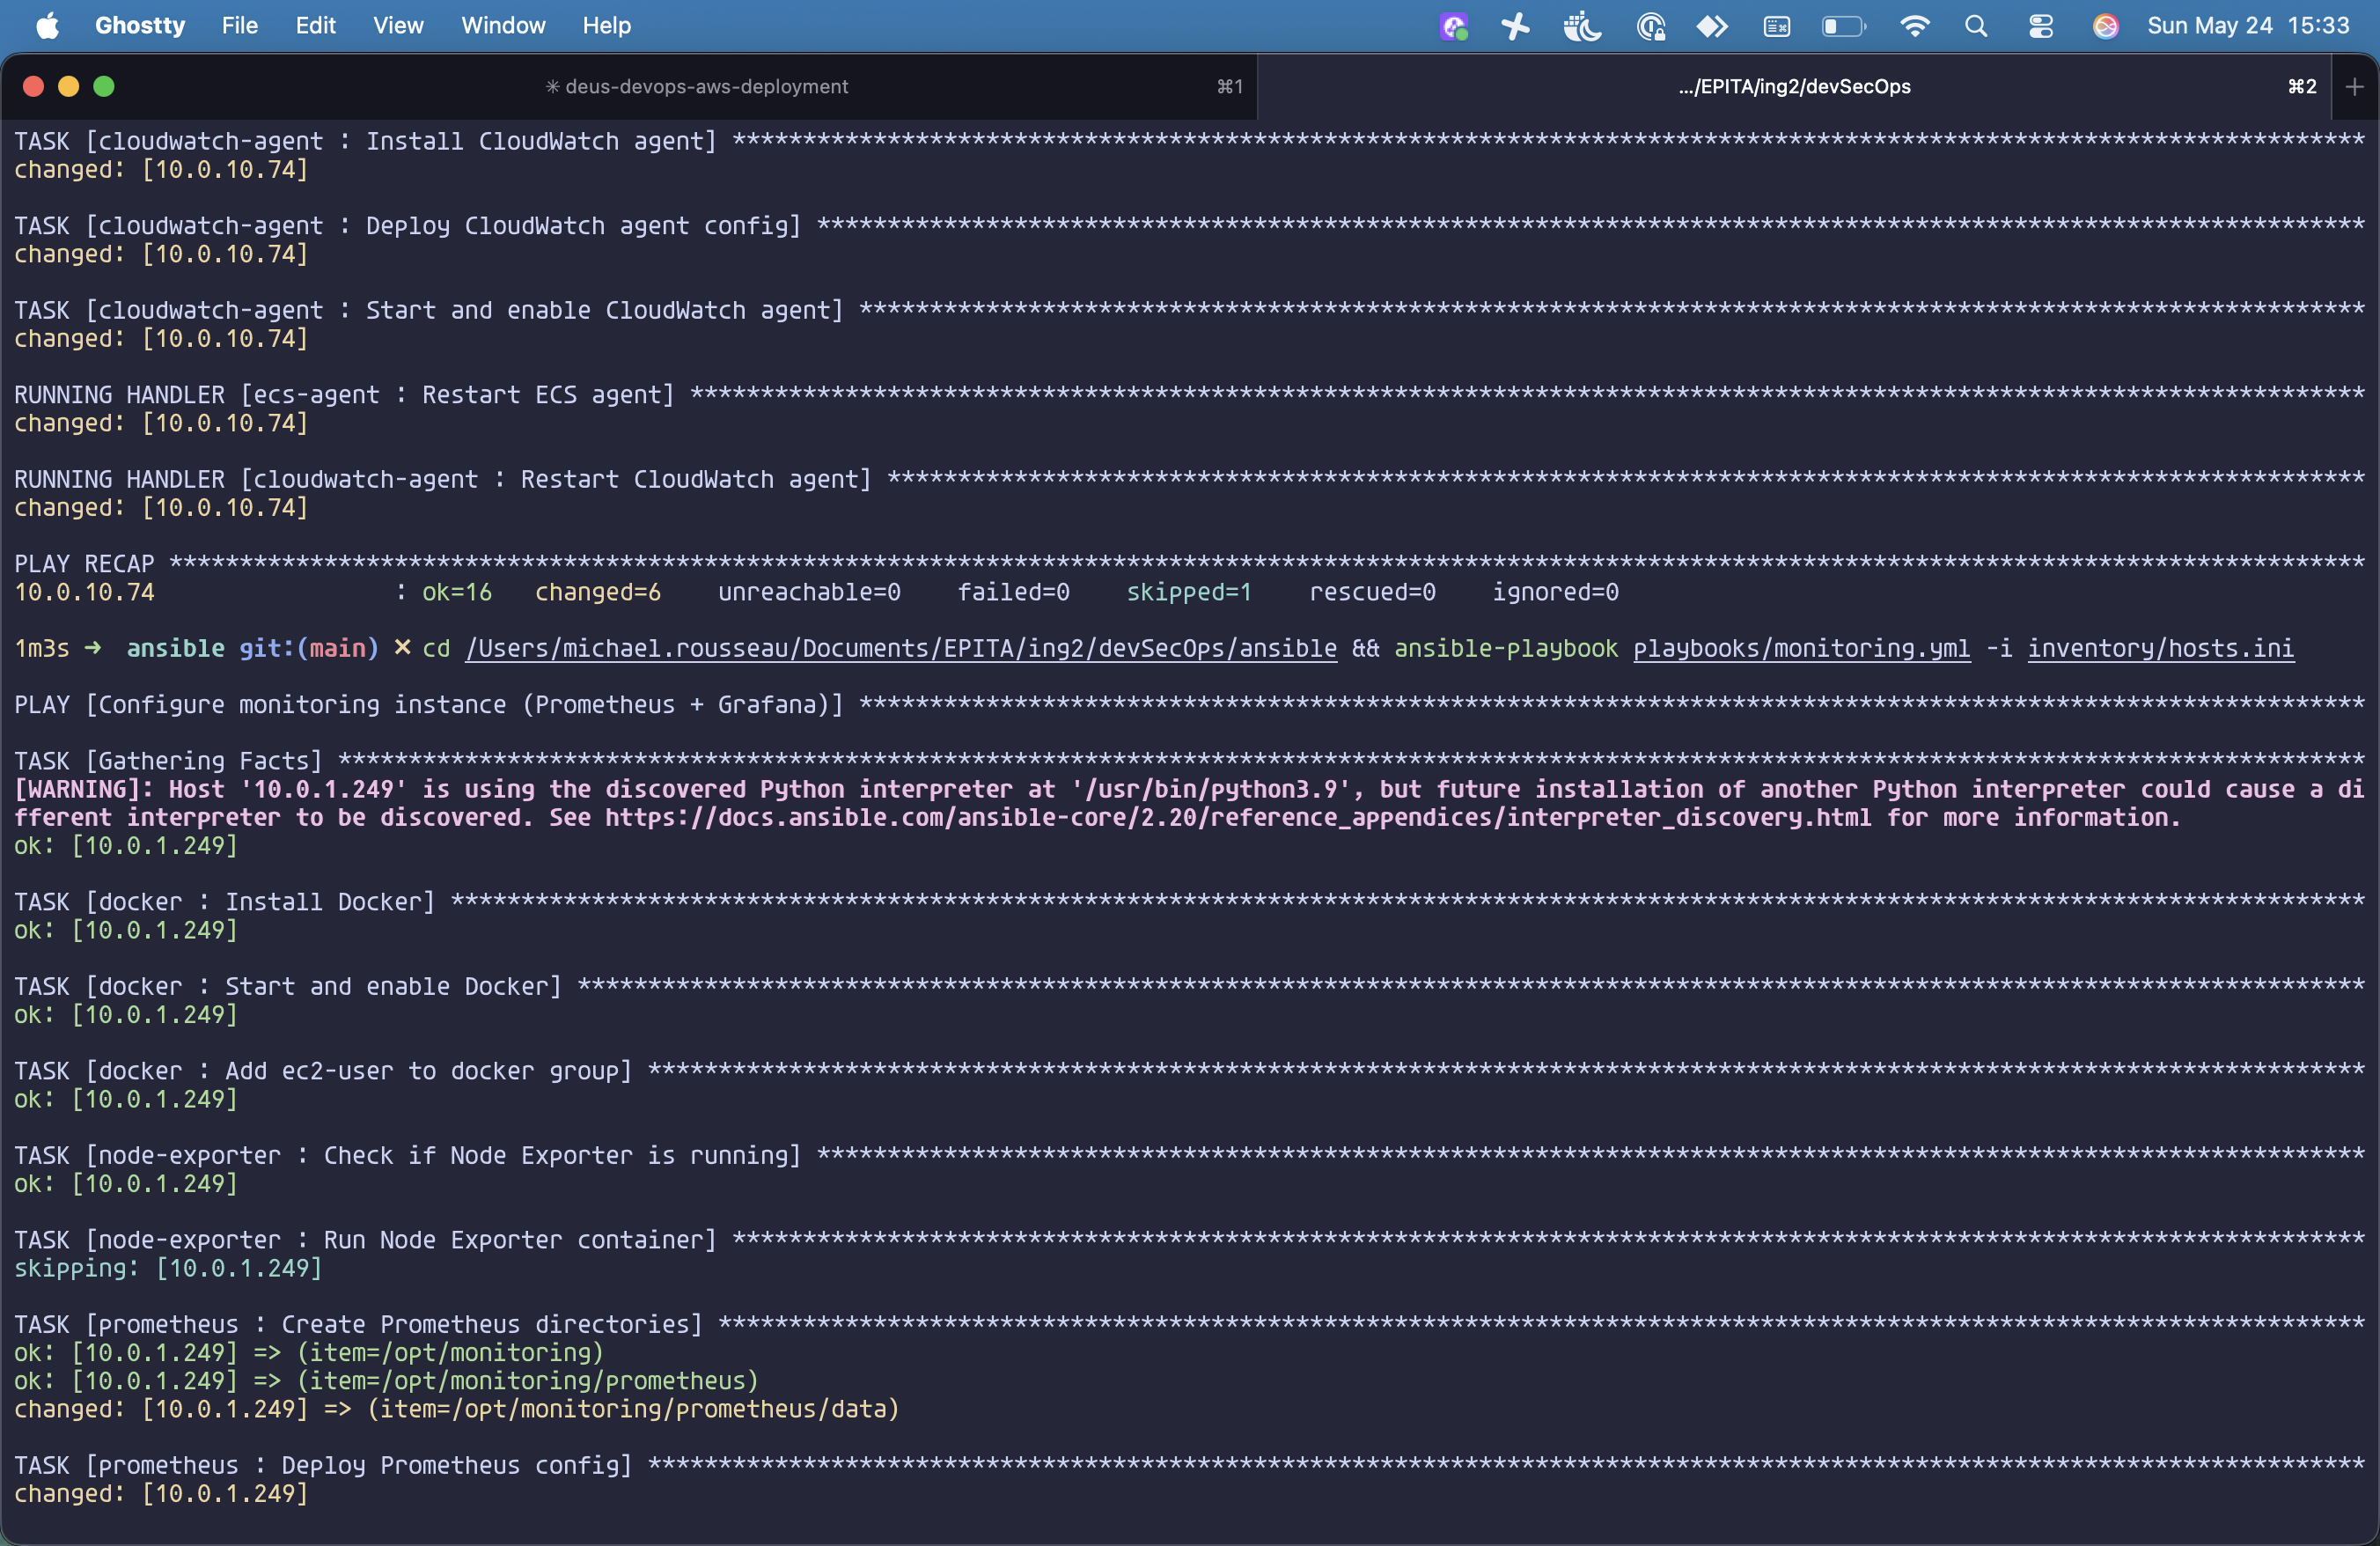
\includegraphics[width=\textwidth]{ansible_init.png}
    \caption{Execution du playbook Ansible}
\end{figure}

\chapter{CI/CD --- GitHub Actions}

\section{Presentation}

Le code source est heberge sur le depot GitHub
\texttt{Michael-Rousseau/devSecOps}\footnote{\texttt{https://github.com/Michael-Rousseau/devSecOps}}.
Quatre workflows GitHub Actions automatisent l'ensemble du cycle de vie~:

\begin{table}[H]
    \centering
    \begin{tabularx}{\textwidth}{lllX}
        \toprule
        \textbf{Workflow} & \textbf{Declencheur} & \textbf{Type} & \textbf{Actions} \\
        \midrule
        ci.yml & PR vers main & CI & Lint, test, build (frontend + backend) \\
        cd-frontend.yml & Push sur main & CD & Build Angular, sync S3 (\texttt{deus-dashboard-frontend-dev}) \\
        cd-backend.yml & Push sur main & CD & Build Docker, push ECR, deploy ECS \\
        terraform.yml & PR / Push & IaC & Plan sur PR, Apply sur merge \\
        \bottomrule
    \end{tabularx}
    \caption{Workflows GitHub Actions}
\end{table}

\section{Pipeline CI}

Le workflow CI s'execute sur chaque Pull Request~:

\begin{lstlisting}[language=bash,caption={Jobs CI en parallele}]
frontend:
  npm ci -> npm run lint -> npm run build

backend:
  cd backend && npm ci -> npm run build
\end{lstlisting}

La concurrence est geree pour annuler les executions obsoletes sur une meme branche.

\section{Deploiement Frontend}

\begin{enumerate}
    \item Build de l'application Angular en mode production
    \item Synchronisation des fichiers vers le bucket S3
        \texttt{deus-dashboard-frontend-dev} via \texttt{aws s3 sync}
\end{enumerate}

\textbf{Note~:} L'etape d'invalidation CloudFront initialement prevue a ete
supprimee car l'hebergement utilise le mode S3 Static Website Hosting
(cf. chapitre~\ref{chap:architecture} --- Adaptations Learner Lab).

\section{Deploiement Backend}

\begin{enumerate}
    \item Build de l'image Docker
    \item Push vers Amazon ECR
        \texttt{459624991030.dkr.ecr.us-east-1.amazonaws.com/deus-dashboard-backend}
        (tag~: SHA du commit + latest)
    \item Mise a jour de la Task Definition ECS sur le cluster
        \texttt{deus-dashboard-dev}
    \item Deploiement du service ECS \texttt{deus-dashboard-backend}
        avec attente de stabilite
\end{enumerate}

\section{Terraform en CI}

\begin{description}
    \item[Sur Pull Request] \texttt{terraform plan} est execute et le resultat
        est poste en commentaire sur la PR pour revue.
    \item[Sur merge vers main] \texttt{terraform apply -auto-approve} est execute
        automatiquement.
\end{description}

\section{Gestion des credentials AWS Learner Lab}

Les credentials AWS Learner Lab (compte \texttt{459624991030}, region
\texttt{us-east-1}) expirent toutes les \~{}4 heures.
Un script \texttt{scripts/update-aws-keys.sh} permet de mettre a jour
simultanement~:
\begin{itemize}
    \item \texttt{\~{}/.aws/credentials} (CLI locale)
    \item Les GitHub Secrets du depot \texttt{Michael-Rousseau/devSecOps}
        (via \texttt{gh secret set})
\end{itemize}

Les trois secrets concernes sont~:
\begin{itemize}
    \item \texttt{AWS\_ACCESS\_KEY\_ID}
    \item \texttt{AWS\_SECRET\_ACCESS\_KEY}
    \item \texttt{AWS\_SESSION\_TOKEN}
\end{itemize}

\textbf{Limitation~:} L'absence de federation OIDC (non autorisee par Learner Lab)
impose l'utilisation de cles statiques dans les GitHub Secrets. Ces cles doivent
etre renouvelees manuellement avant chaque session de deploiement. En production,
on privilegierait un provider OIDC
(\texttt{aws-actions/configure-aws-credentials}) pour eviter le stockage de cles
longue duree.

\begin{figure}[H]
    \centering
    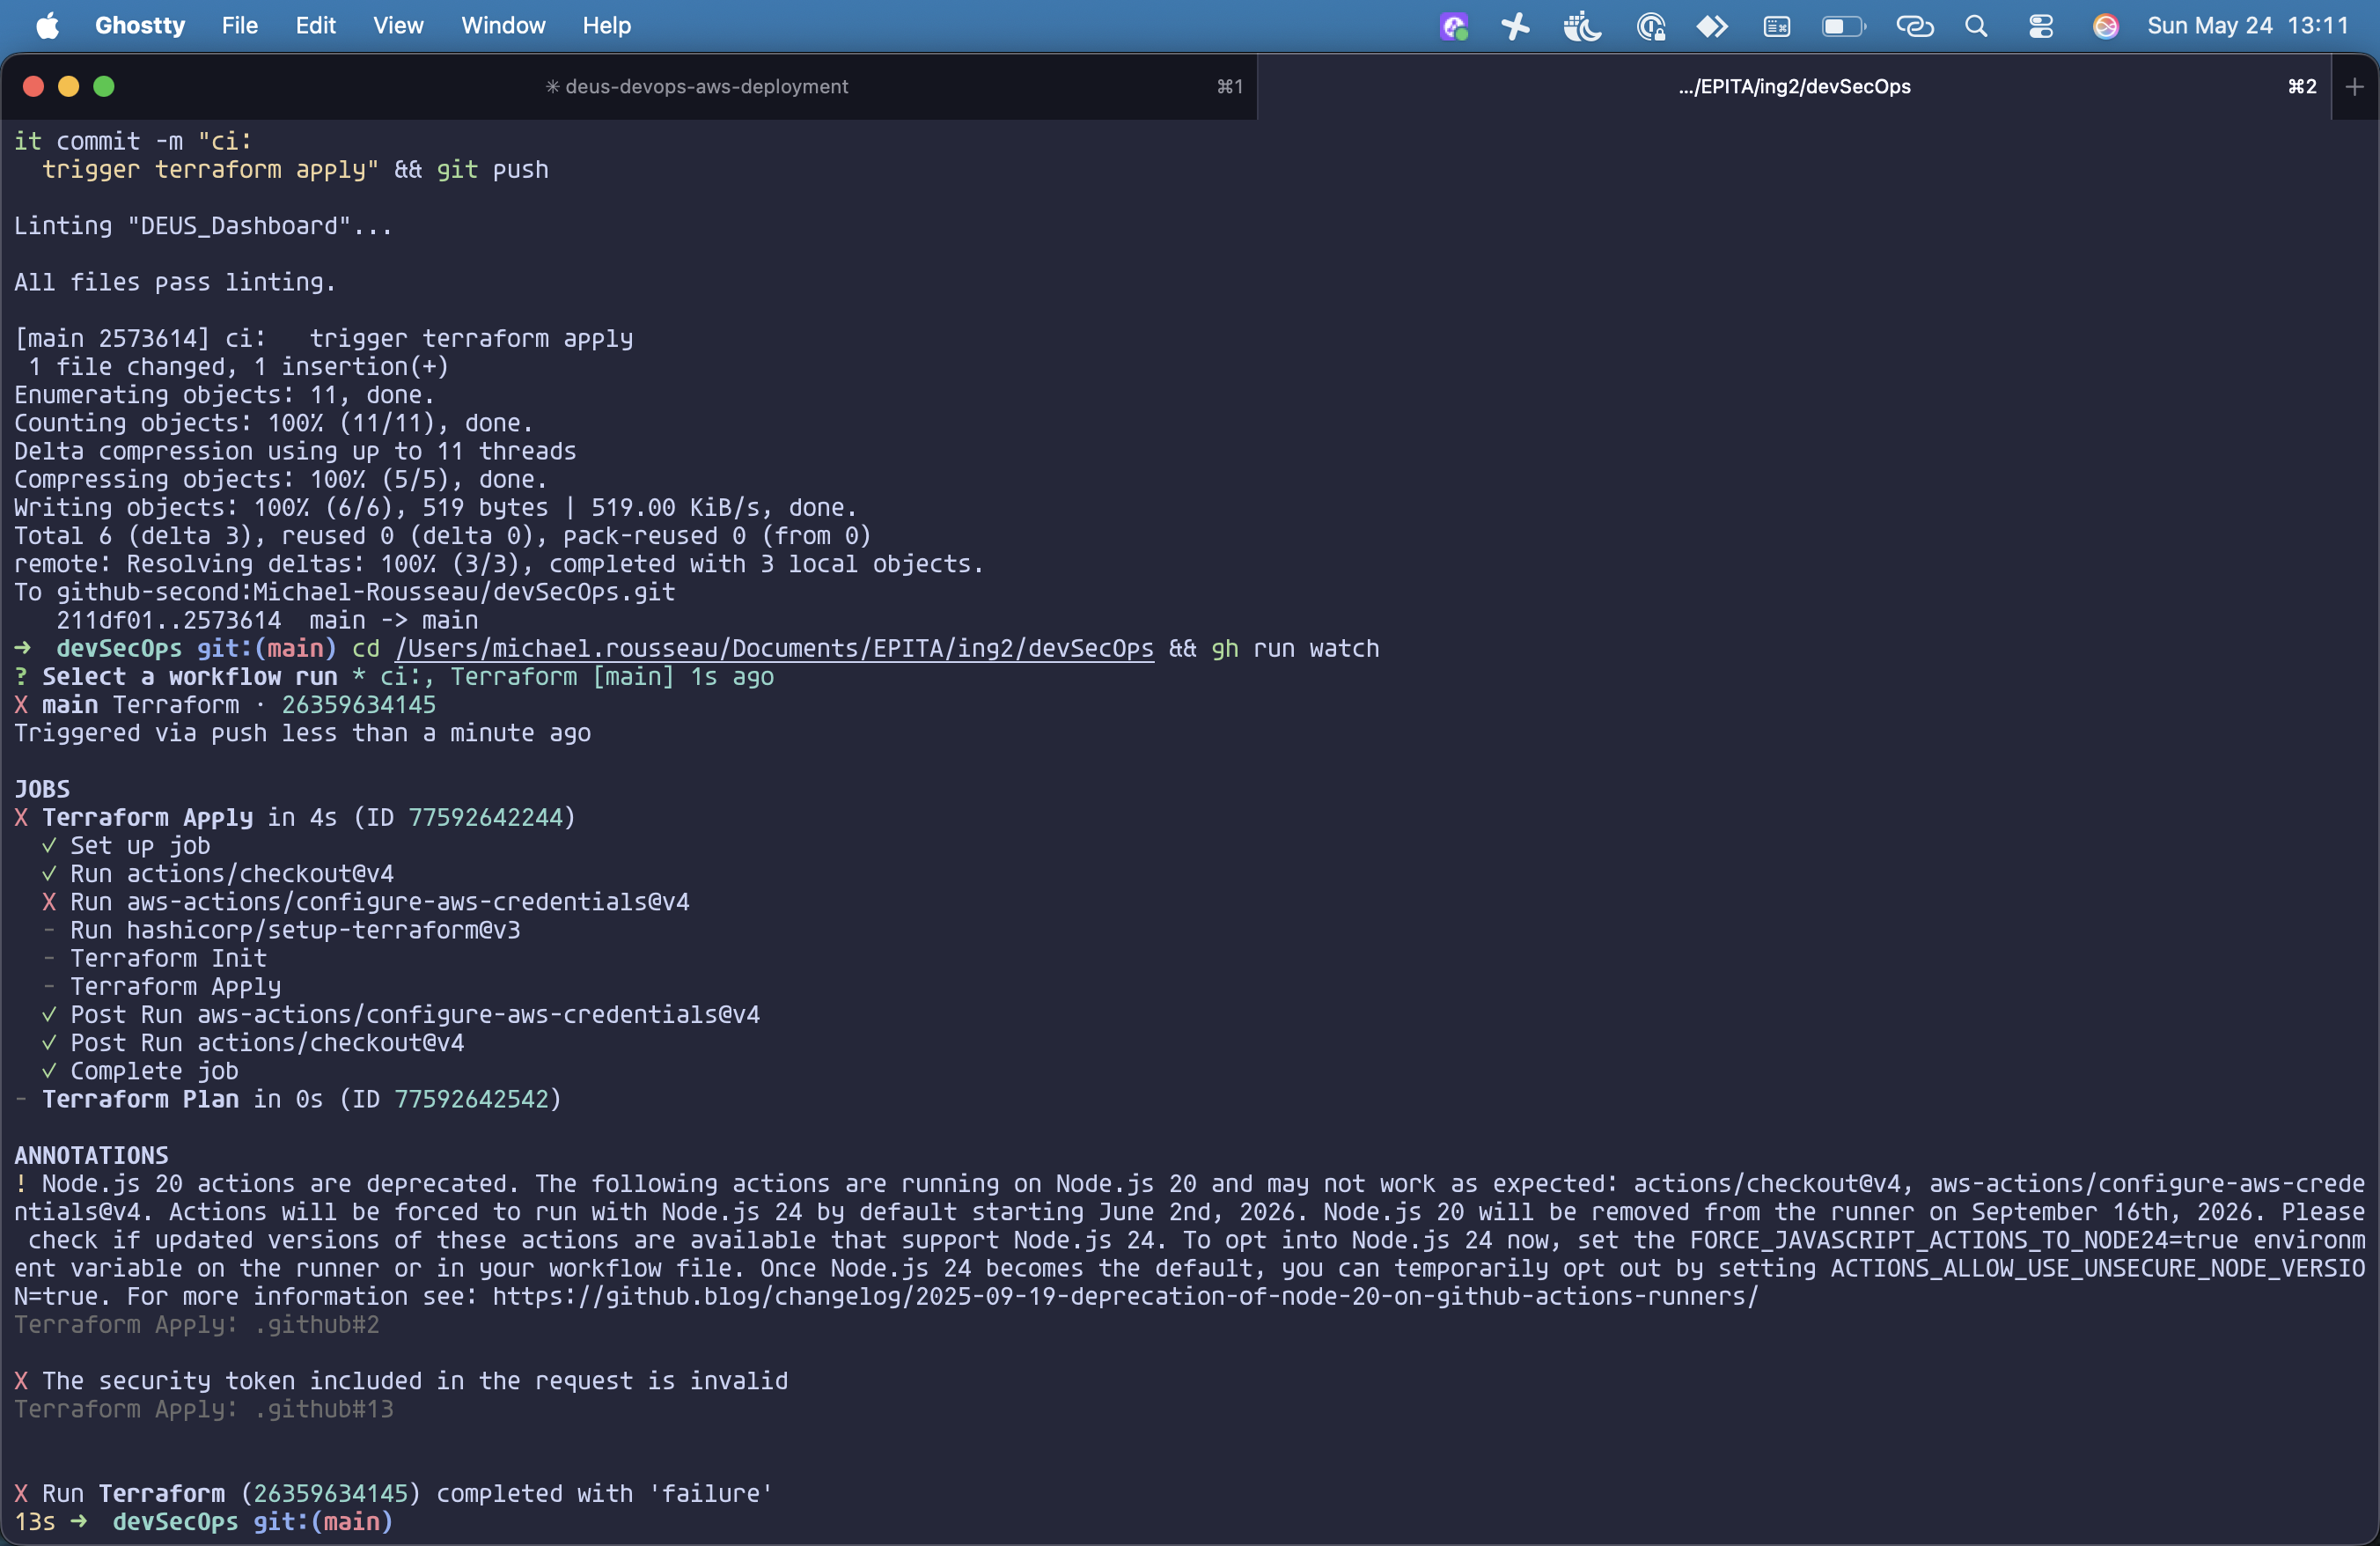
\includegraphics[width=\textwidth]{gh_watch_ci.png}
    \caption{Pipeline CI sur une Pull Request}
\end{figure}

\chapter{Monitoring et Logging}

\section{Presentation}

Le monitoring repose sur trois piliers complementaires~:
\begin{itemize}
    \item \textbf{CloudWatch} --- Monitoring AWS natif (logs, metriques, alarmes)
    \item \textbf{Prometheus + Grafana} --- Metriques applicatives et dashboards personnalises
    \item \textbf{SonarQube} --- Qualite du code et analyse statique
\end{itemize}

\section{CloudWatch}

\subsection{Logs}

Les conteneurs ECS emettent leurs logs via le driver \texttt{awslogs}
vers le groupe \texttt{/ecs/deus-dashboard-backend} avec une retention de 14 jours.
L'agent CloudWatch (installe par Ansible) collecte egalement les logs de l'agent ECS.

\subsection{Alarmes}

\begin{table}[H]
    \centering
    \begin{tabularx}{\textwidth}{lXl}
        \toprule
        \textbf{Alarme} & \textbf{Condition} & \textbf{Action} \\
        \midrule
        ECS CPU elevee & CPU > 80\% pendant 10 min & Email SNS \\
        ECS memoire elevee & Memoire > 80\% pendant 10 min & Email SNS \\
        ALB erreurs 5xx & > 10 erreurs en 5 min & Email SNS \\
        RDS CPU elevee & CPU > 80\% pendant 10 min & Email SNS \\
        RDS stockage bas & < 2 Go restants & Email SNS \\
        \bottomrule
    \end{tabularx}
    \caption{Alarmes CloudWatch configurees}
\end{table}

\section{Prometheus}

Prometheus est deploye sur une instance EC2 dediee au monitoring
(\texttt{34.207.159.92}), accessible a l'adresse
\texttt{http://34.207.159.92:9090}.
Il collecte les metriques via le protocole pull (scraping)~:

\begin{table}[H]
    \centering
    \begin{tabularx}{\textwidth}{llX}
        \toprule
        \textbf{Job} & \textbf{Cible} & \textbf{Metriques} \\
        \midrule
        deus-backend & ALB:80/api/metrics & Requetes HTTP (duree, compteur), cache hits/miss, heap Node.js \\
        node-exporter & localhost:9100 & CPU, memoire, disque, reseau de l'instance \\
        prometheus & localhost:9090 & Metriques internes de Prometheus \\
        \bottomrule
    \end{tabularx}
    \caption{Jobs de scraping Prometheus}
\end{table}

\subsection{Metriques applicatives}

Le backend expose un endpoint \texttt{/api/metrics} au format Prometheus
grace a la librairie \texttt{prom-client}~:

\begin{lstlisting}[language=bash,caption={Metriques exposees par le backend}]
# Duree des requetes HTTP (histogramme)
http_request_duration_seconds_bucket{method,route,status_code}

# Compteur total de requetes
http_requests_total{method,route,status_code}

# Hits et miss du cache DynamoDB
cache_hit_total{route}
cache_miss_total{route}

# Metriques Node.js par defaut
nodejs_heap_size_used_bytes
nodejs_active_handles_total
process_cpu_user_seconds_total
\end{lstlisting}

\section{Grafana}

Grafana est deploye sur la meme instance que Prometheus
(\texttt{http://34.207.159.92:3000}) et fournit des dashboards interactifs.

\subsection{Sources de donnees}

\begin{itemize}
    \item \textbf{Prometheus} --- Metriques applicatives et systeme
    \item \textbf{CloudWatch} --- Metriques AWS (ECS, ALB, RDS)
\end{itemize}

\subsection{Dashboard Backend Overview}

Le dashboard pre-provisionne comprend~:
\begin{itemize}
    \item Taux de requetes par seconde (par methode, route, code de statut)
    \item Latence des requetes (percentiles p50 et p95)
    \item Taux de hit du cache DynamoDB (jauge)
    \item Taux d'erreurs 5xx
    \item Utilisation CPU et memoire de l'instance (via Node Exporter)
    \item Utilisation du heap Node.js
\end{itemize}

\subsection{Acces au monitoring}

\begin{table}[H]
    \centering
    \begin{tabular}{lll}
        \toprule
        \textbf{Service} & \textbf{URL} & \textbf{Port} \\
        \midrule
        Grafana & \texttt{http://34.207.159.92:3000} & 3000 \\
        Prometheus & \texttt{http://34.207.159.92:9090} & 9090 \\
        Node Exporter & \texttt{http://34.207.159.92:9100} & 9100 \\
        \bottomrule
    \end{tabular}
    \caption{URLs d'acces aux services de monitoring}
\end{table}

% TODO: Capture d'ecran du dashboard Grafana
% \begin{figure}[H]
%     \centering
%     \includegraphics[width=\textwidth]{grafana-dashboard.png}
%     \caption{Dashboard Grafana --- Backend Overview}
% \end{figure}

\section{SonarQube --- Qualite du code}

SonarQube analyse le code source pour detecter~:
\begin{itemize}
    \item Les bugs potentiels
    \item Les vulnerabilites de securite
    \item Le code duplique
    \item Les code smells (mauvaises pratiques)
    \item La couverture de tests
\end{itemize}

\subsection{Integration CI}

L'analyse SonarQube s'execute automatiquement dans le pipeline CI
(GitHub Actions) apres les etapes de build. Le fichier
\texttt{sonar-project.properties} configure les sources a analyser~:

\begin{lstlisting}[language=bash,caption={Configuration SonarQube}]
sonar.projectKey=deus-dashboard
sonar.sources=src,backend/src
sonar.exclusions=**/node_modules/**,**/dist/**
\end{lstlisting}

\subsection{Developpement local}

SonarQube est egalement disponible en local via Docker Compose
sur le port 9000 (\texttt{http://localhost:9000}).

% TODO: Capture d'ecran SonarQube
% \begin{figure}[H]
%     \centering
%     \includegraphics[width=\textwidth]{sonarqube-dashboard.png}
%     \caption{Dashboard SonarQube}
% \end{figure}

\section{Architecture du monitoring}

\begin{lstlisting}[language={},caption={Flux de monitoring}]
   Backend (ECS) --scrape--> Prometheus
                 --awslogs--> CloudWatch
                 --sonar-scan--> SonarQube (CI)

   Node Exporter --scrape--> Prometheus

   Prometheus --> Grafana (dashboards)
   CloudWatch --> Grafana (datasource)
   CloudWatch --> SNS --> Email (alarmes)
\end{lstlisting}

\chapter{Securite}

\section{Gestion des secrets --- SSM Parameter Store}

Les secrets sont stockes dans AWS Systems Manager Parameter Store
en tant que \texttt{SecureString} (chiffres avec KMS)~:

\begin{table}[H]
    \centering
    \begin{tabularx}{\textwidth}{lXl}
        \toprule
        \textbf{Parametre} & \textbf{Usage} & \textbf{Type} \\
        \midrule
        /deus-dashboard/dev/nasa-api-key & Cle API NASA & SecureString \\
        /deus-dashboard/dev/pg-host & Adresse RDS & String \\
        /deus-dashboard/dev/pg-password & Mot de passe DB & SecureString \\
        /deus-dashboard/dev/dynamodb-table & Nom de la table & String \\
        \bottomrule
    \end{tabularx}
    \caption{Parametres SSM}
\end{table}

Le role d'execution ECS lit ces parametres au demarrage du conteneur
et les injecte comme variables d'environnement.

\section{IAM --- Adaptations Learner Lab}

\subsection{Architecture cible vs. realite Learner Lab}

L'architecture ideale prevoyait trois roles IAM distincts suivant le
principe du moindre privilege~:

\begin{description}
    \item[Execution Role] Permettrait a ECS de~: tirer des images ECR,
        lire les parametres SSM, ecrire dans CloudWatch Logs.
    \item[Task Role] Permettrait au conteneur de~: acceder a DynamoDB
        (lecture/ecriture sur la table de cache).
    \item[Instance Role] Permettrait aux instances EC2 de~: s'enregistrer
        au cluster ECS, utiliser SSM Session Manager, envoyer des metriques CloudWatch.
\end{description}

\subsection{Contrainte Learner Lab}

L'environnement AWS Academy Learner Lab interdit la creation de roles IAM
(\texttt{iam:CreateRole} non autorise). En consequence, l'ensemble des
ressources utilisent le role pre-existant \textbf{LabRole}, qui dispose
de permissions larges couvrant les services necessaires (ECS, ECR, SSM,
CloudWatch, DynamoDB, S3, RDS).

\begin{lstlisting}[language=bash,caption={Utilisation du LabRole dans Terraform}]
# Au lieu de creer des roles personnalises
data "aws_iam_role" "lab_role" {
  name = "LabRole"
}

# Execution role et task role ECS
execution_role_arn = data.aws_iam_role.lab_role.arn
task_role_arn      = data.aws_iam_role.lab_role.arn

# Instance profile pour les EC2 (ECS, bastion)
data "aws_iam_instance_profile" "lab_profile" {
  name = "LabInstanceProfile"
}
\end{lstlisting}

\textbf{Compromis de securite~:} Le \texttt{LabRole} dispose de permissions
plus larges que necessaire, ce qui contrevient au principe du moindre privilege.
En environnement de production, on creerait des roles specifiques avec des
politiques restrictives pour chaque composant.

\section{Reseau --- Segmentation VPC}

\begin{table}[H]
    \centering
    \begin{tabularx}{\textwidth}{lXl}
        \toprule
        \textbf{Security Group} & \textbf{Regles entrantes} & \textbf{Cible} \\
        \midrule
        sg-alb & 80 depuis 0.0.0.0/0 & ALB \\
        sg-ecs & 32768-65535 depuis sg-alb, 22 depuis sg-bastion & Instances ECS \\
        sg-rds & 5432 depuis sg-ecs et sg-bastion & PostgreSQL \\
        sg-bastion & 22 depuis IP autorisee & Bastion \\
        sg-monitoring & 3000/9090 depuis IP autorisee, 22 depuis sg-bastion & Prometheus/Grafana \\
        \bottomrule
    \end{tabularx}
    \caption{Security Groups et regles}
\end{table}

\textbf{Moindre privilege par references de Security Groups~:} chaque flux
interne est autorise par \emph{reference de Security Group} et non par plage
CIDR. Initialement, la base RDS acceptait le port 5432 depuis l'ensemble des
sous-reseaux prives~; la regle a ete restreinte aux seuls
\texttt{sg-ecs} et \texttt{sg-bastion}. Ainsi, meme une ressource compromise
placee dans un sous-reseau prive ne peut pas atteindre la base si elle ne
porte pas le bon Security Group. De meme, le port 443 de l'ALB, sans
listener HTTPS associe (certificat ACM indisponible en Learner Lab),
a ete supprime~: aucune regle ne reste ouverte sans service derriere.

Les flux autorises se resument a~:
\begin{lstlisting}[language={},caption={Flux reseau (moindre privilege)}]
Internet --80--> sg-alb --ports dynamiques--> sg-ecs --5432--> sg-rds
Admin    --22--> sg-bastion --22--> sg-ecs / sg-monitoring
                 sg-bastion --5432--> sg-rds   (administration DB)
Admin    --3000/9090--> sg-monitoring          (UI Grafana/Prometheus)
\end{lstlisting}

Seul l'ALB est expose sur Internet. Les instances ECS et la base de donnees
sont dans des sous-reseaux prives, accessibles uniquement via l'ALB
ou le bastion SSH.

\section{Bastion SSH}

Le bastion est le point d'entree unique pour l'acces SSH aux ressources privees.
Il est configure avec~:
\begin{itemize}
    \item Acces SSH restreint a l'IP de l'administrateur
    \item Instance \texttt{t2.micro} (Free Tier)
    \item Durcissement via Ansible (pas de root SSH, pas d'authentification par mot de passe)
\end{itemize}

\section{Cle API NASA}

La cle API NASA, auparavant codee en dur dans le code source Angular
(visible dans le navigateur), est desormais~:
\begin{enumerate}
    \item Stockee dans SSM Parameter Store (chiffree)
    \item Injectee dans le conteneur backend via la Task Definition ECS
    \item Utilisee cote serveur uniquement --- le frontend ne la voit plus
\end{enumerate}

\chapter{Procedure de deploiement}

\section{Prerequis}

\begin{itemize}
    \item Compte AWS Learner Lab actif
    \item CLI AWS, Terraform, Ansible et Docker installes localement
    \item Repository GitHub avec les secrets configures
    \item Paire de cles SSH (key pair) creee dans la console AWS
\end{itemize}

\section{Etape 1 --- Initialisation des credentials}

\begin{lstlisting}[language=bash,caption={Rotation des cles Learner Lab}]
# Executer le script de rotation
./scripts/update-aws-keys.sh

# Verifier l'acces
aws sts get-caller-identity
\end{lstlisting}

\textbf{Important~:} Les credentials Learner Lab expirent toutes les \~{}4 heures.
Le script met a jour \texttt{\~{}/.aws/credentials} et optionnellement les GitHub Secrets.

\section{Etape 2 --- Bootstrap Terraform}

\begin{lstlisting}[language=bash,caption={Creation du bucket d'etat}]
cd terraform/bootstrap
terraform init
terraform apply
\end{lstlisting}

Cette etape cree le bucket S3 et la table DynamoDB pour le state Terraform.
Elle n'est executee qu'une seule fois.

\section{Etape 3 --- Deploiement de l'infrastructure}

\begin{lstlisting}[language=bash,caption={Deploiement complet}]
cd terraform/environments/dev
terraform init
terraform plan -var="db_password=<MOT_DE_PASSE>" \
               -var="nasa_api_key=<CLE_NASA>" \
               -var="ssh_key_name=<NOM_KEY_PAIR>"
terraform apply
\end{lstlisting}

\section{Etape 4 --- Configuration Ansible}

\begin{lstlisting}[language=bash,caption={Execution d'Ansible}]
cd ansible
# Mettre a jour l'IP du bastion dans la config SSH
ansible-playbook playbooks/site.yml
\end{lstlisting}

\section{Etape 5 --- Premier deploiement applicatif}

\begin{lstlisting}[language=bash,caption={Build et push de l'image Docker}]
# Backend
cd backend
aws ecr get-login-password | docker login --username AWS \
  --password-stdin <ECR_URL>
docker build -t <ECR_URL>:latest .
docker push <ECR_URL>:latest

# Frontend
cd ..
npm run build
aws s3 sync dist/DEUS_Dashboard/browser/ s3://<BUCKET> --delete
aws cloudfront create-invalidation \
  --distribution-id <CF_ID> --paths "/*"
\end{lstlisting}

\section{Etape 6 --- Verification}

\begin{enumerate}
    \item Acceder au domaine CloudFront --- l'application Angular doit s'afficher
    \item Verifier que l'APOD se charge (appel via le backend)
    \item Tester la liste des evenements naturels
    \item Consulter le dashboard CloudWatch
    \item Verifier les logs dans le groupe \texttt{/ecs/deus-dashboard-backend}
\end{enumerate}

\section{Gestion des sessions Learner Lab}

\begin{table}[H]
    \centering
    \begin{tabularx}{\textwidth}{lX}
        \toprule
        \textbf{Emplacement} & \textbf{Action requise} \\
        \midrule
        \texttt{\~{}/.aws/credentials} & Executer \texttt{update-aws-keys.sh} \\
        GitHub Secrets & Repondre ``y'' dans le script \\
        Backend S3 Terraform & Utilise les memes credentials CLI \\
        \bottomrule
    \end{tabularx}
    \caption{Points de mise a jour des credentials}
\end{table}

% TODO: Captures d'ecran du deploiement
% \begin{figure}[H]
%     \centering
%     \includegraphics[width=\textwidth]{deploy-cloudfront.png}
%     \caption{Application deployee sur CloudFront}
% \end{figure}

\chapter{Conclusion}

\section{Bilan technique}

Ce projet a permis de mettre en \oe{}uvre une chaine DevOps complete,
couvrant l'ensemble du cycle de vie d'une application web~:

\begin{itemize}
    \item \textbf{Conteneurisation} --- Docker pour l'isolation et la reproductibilite
    \item \textbf{Infrastructure as Code} --- Terraform avec 10 modules couvrant VPC,
        ECS, RDS, DynamoDB, S3/CloudFront, IAM, SSM, et le monitoring
    \item \textbf{Configuration Management} --- Ansible avec 4 roles pour la configuration
        automatisee des instances EC2
    \item \textbf{CI/CD} --- GitHub Actions avec 4 workflows (CI, deploiement frontend,
        deploiement backend, Terraform plan/apply)
    \item \textbf{Monitoring} --- CloudWatch avec logs, metriques, alarmes et dashboard
    \item \textbf{Securite} --- IAM least-privilege, VPC segmente, SSM pour les secrets,
        bastion SSH
\end{itemize}

\section{Difficultes rencontrees}

\begin{itemize}
    \item \textbf{Credentials Learner Lab} --- L'expiration toutes les 4 heures
        necessite une rotation frequente, resolue par le script automatise
    \item \textbf{Dependances circulaires Terraform} --- Le module RDS avait besoin
        du Security Group ECS, qui dependait de SSM, qui dependait de RDS.
        Resolution~: utilisation de CIDR blocks au lieu de references de Security Groups
    \item \textbf{Dimensionnement ECS} --- Les instances \texttt{t3.micro} ne disposent
        pas de suffisamment de memoire pour l'agent ECS et les conteneurs.
        Solution~: utilisation de \texttt{t2.small}
\end{itemize}

\section{Ameliorations possibles}

\begin{itemize}
    \item \textbf{HTTPS} --- Ajout d'un certificat ACM avec un nom de domaine personnalise
    \item \textbf{Auto Scaling} --- Policies de scaling automatique basees sur la charge
    \item \textbf{Multi-environnement} --- Separation dev/staging/prod avec des workspaces
        Terraform
    \item \textbf{Authentification} --- Integration d'Amazon Cognito pour l'authentification
        utilisateur
    \item \textbf{Migration Fargate} --- Pour eliminer la gestion des instances EC2
        en production
    \item \textbf{Prometheus/Grafana} --- Pour un monitoring plus avance avec des dashboards
        personnalises
\end{itemize}


\printbibliography[heading=bibintoc,title={References}]

\end{document}
